\documentclass[10pt]{article}
\usepackage[polish]{babel}
\usepackage[utf8]{inputenc}
\usepackage[T1]{fontenc}
\usepackage{amsmath}
\usepackage{amsfonts}
\usepackage{amssymb}
\usepackage[version=4]{mhchem}
\usepackage{stmaryrd}
\usepackage{graphicx}
\usepackage[export]{adjustbox}
\graphicspath{ {./images/} }

\title{Kod ucznia }

\author{}
\date{}


\begin{document}
\maketitle
\(\qquad\) Nazwisko i imię \(\qquad\)

\section*{\(\square\) \\
 MATEMATYKA}
\section*{Instrukcja dla zdającego}
Czas pracy:\\
180 minut

\begin{enumerate}
  \item Sprawdź, czy arkusz zawiera 16 stron (zadania 1-16). Ewentualny brak zgłoś przewodniczącemu zespołu nadzorującego egzamin.
  \item Rozwiązania zadań i odpowiedzi zamieść w miejscu na to przeznaczonym.
  \item Odpowiedzi do zadań zamkniętych (1-5) przenieś na kartę odpowiedzi, zaznaczając je w części karty przeznaczonej dla zdającego. Zamaluj pola do tego przeznaczone. Błędne zaznaczenie otocz kółkiem i zaznacz właściwe.
  \item Pamiętaj, że pominięcie argumentacji lub istotnych obliczeń w rozwiązaniu zadania otwartego (7-16) może spowodować, że za to rozwiązanie nie otrzymasz pełnej liczby punktów.
  \item Pisz czytelnie i używaj tylko dlugopisu lub pióra z czarnym tuszem lub atramentem.
  \item Nie używaj korektora, a błędne zapisy wyraźnie przekreśl.
  \item Pamiętaj, że zapisy w brudnopisie nie będą oceniane.
  \item Możesz korzystać z zestawu wzorów matematycznych, cyrkla i linijki oraz kalkulatora prostego.
  \item Na tej stronie oraz na karcie odpowiedzi wpisz swój kod (nazwisko i imię - zgodnie z ustaleniami szkolnymi).
  \item Nie wpisuj żadnych znaków w części przeznaczonej dla egzaminatora.
\end{enumerate}

Życzymy powodzenia!\\
Liczba punktów\\
do uzyskania: \(\mathbf{5 0}\)

W zadaniach o numerach od 1 do 5 wybierz i zaznacz na karcie odpowiedzi jedną poprawną odpowiedź

\section*{Zadanie 1. (1pkt)}
Wzór funkcji liniowej, której wykresem jest prosta nachylona do osi Ox pod kątem o mierze \(120^{\circ}\) i przechodzi przez punkt \(\mathrm{P}=(-4,2)\) jest postaci:\\
A. \(y=-\sqrt{3} x+2-4 \sqrt{3}\)\\
B. \(y=-\sqrt{3} x+2+4 \sqrt{3}\)\\
C. \(y=-\sqrt{3} x-2-4 \sqrt{3}\)\\
D. \(y=\sqrt{3} x+2-4 \sqrt{3}\)

Zadanie 2. (1pkt)\\
Do okręgu należą punkty \(A=(2,1) ; B=(5,0) ; C=(4,-3)\). Jest to okrąg o środku \(S\) i promieniu r :\\
A. \(S=(2,-2) r=\sqrt{2}\)\\
B. \(S=(3,-1) r=\sqrt{5}\)\\
C. \(S=(3,0) r=1\)\\
D. \(S=(2,-2) r=3\)

\section*{Zadanie 3. (1pkt)|}
Funkcja \(f(x)=\left\{\begin{array}{lll}a^{2} x-a & g d y & x \in(-\infty ; 5) \\ 10 a x-46 & g d y & x \in\langle 5 ; \infty)\end{array}\right.\) jest ciągła w zbiorze liczb rzeczywistych jeżeli \(\boldsymbol{a}\) jest równe:\\
A. \(1 \operatorname{lub} 9 \frac{1}{5}\)\\
B. 5 lub \(3 \frac{1}{9}\)\\
C. 5 lub \(-3 \frac{1}{9}\)\\
D. 1 lub 5

\section*{Zadanie 4. (1pkt)}
Ile różnych wyrazów z sensem lub bez sensu można ułożyć z liter wyrazu:

\section*{MATEMATYKA}
A. 10 !\\
B. 30240\\
C. 151200\\
D. \(3!2!2\) !

Zadanie 5. (1pkt)\\
Rozwiązaniem nierówności \(||x-1|-3| \geq 4\) jest:\\
A. \(x \in(-\infty ;-6\rangle \cup\langle 8 ; \infty)\)\\
B. \(x \in(-\infty ;-8) \cup(6 ; \infty)\)\\
C. \(x \in R\)\\
D. \(x \in\langle-6 ; 8\rangle\)\\

\includegraphics[max width=\textwidth, center]{2024_11_21_498389c978c770348ebcg-03}

W zadaniu 6 zakoduj we wskazanym miejscu wynik zgodnie z poleceniem.

\section*{Zadanie 6. (2pkt)}
Wyznacz zbiór argumentów, dla których funkcja f określona wzorem\\
\(f(x)=\log _{3} x^{2}+\log _{3} x+\log _{\frac{1}{3}} x\) przyjmuje wartości z przedziału \(\langle 6,10\rangle\). Zakoduj wynik, podając średnią arytmetyczną końców otrzymanego przedziału liczbowego.

\begin{center}
\begin{tabular}{|l|l|l|}
\hline
setki & dziesiątki & jedności \\
\hline
 &  &  \\
\hline
\end{tabular}
\end{center}

\begin{center}

\includegraphics[max width=\textwidth]{2024_11_21_498389c978c770348ebcg-04}
\end{center}

Rozwiązania zadań od 7 do 16 należy zapisać w wyznaczonych miejscach pod treścią zadania.

\section*{Zadanie 7. (5pkt)}
W rombie ABCD , którego pole jest równe 10 dane są przeciwległe wierzchołki \(\mathrm{A}(0,4) \mathrm{i} C(4,2)\). Wyznacz pozostałe wierzchołki.\\

\includegraphics[max width=\textwidth, center]{2024_11_21_498389c978c770348ebcg-05}

\section*{Zadanie 8. (5p).}
Wiadomo, że liczby \(3^{2 a}+3, \frac{3^{a}+1}{3}, \frac{4}{8 \cdot 3^{a}+3}\) są odpowiednio pierwszym, drugim i trzecim wyrazem nieskończonego ciągu geometrycznego. Wyznacz a. Dla wyznaczonej wartości a zapisz wzór tego ciągu i oblicz sumę jego wszystkich wyrazów.\\

\includegraphics[max width=\textwidth, center]{2024_11_21_498389c978c770348ebcg-06}

Zadanie 9. (2p).\\
Wykaż, że jeśli \(\mathrm{a}+\mathrm{b}+\mathrm{c}=0\), to \(\frac{a^{3}+b^{3}+c^{3}}{3}=a b c\).\\

\includegraphics[max width=\textwidth, center]{2024_11_21_498389c978c770348ebcg-07}

Zadanie 10. (4p).\\
Wyznacz wszystkie wartości parametru m , dla których równanie \(\sin 2 \mathrm{x}+\mathrm{m} \cos \mathrm{x}=0\) ma w przedziale \(\langle 0, \pi\rangle\) trzy rozwiązania.\\

\includegraphics[max width=\textwidth, center]{2024_11_21_498389c978c770348ebcg-08}

Zadanie 11. (2p).\\
Dany jest trójkąt prostokątny równoramienny ABC. Punkty D i E dzielą przeciwprostokątną AB na trzy odcinki równej długości. Oblicz cosinus kąta DCE.\\

\includegraphics[max width=\textwidth, center]{2024_11_21_498389c978c770348ebcg-09}

Zadanie 12. (3p).\\
Dana jest parabola o równaniu \(y=\frac{1}{4} x^{2}\) i punkt \(\mathrm{F}(0,1)\). Wykaż, że każdy punkt leżący na paraboli jest równo oddalony od punktu F i prostej 1 o równaniu \(\mathrm{y}=-1\).

Zadanie 13. (5p).\\
Wyznacz miejsca zerowe funkcji \(f(x)=\log _{2}\left(-x^{3}-4 x^{2}+3 x+18\right)-\log _{2}\left(-2 x^{2}-2 x+12\right)\).\\

\includegraphics[max width=\textwidth, center]{2024_11_21_498389c978c770348ebcg-11}

Zadanie 14. (6p).\\
Punkt \(\mathrm{P}(1,7)\) należy do wykresu funkcji \(f(x)=\frac{x^{2}+a x+5}{x+b}\), gdzie \(b \neq-1\).\\
Styczna do wykresu funkcji fw punkcie P jest prostopadła do prostej o równaniu \(2 \mathrm{x}+3 \mathrm{y}=0\). Oblicz współczynniki a i b oraz napisz równanie tej stycznej.\\

\includegraphics[max width=\textwidth, center]{2024_11_21_498389c978c770348ebcg-12}

Zadanie 15. (4p).\\
Ze zboru \(\{0,1,2,3,4, \ldots ., 2 \mathrm{n}\}\) gdzie \(n \in N\) wylosowano jednocześnie 3 liczby.\\
Prawdopodobieństwo, że suma wylosowanych liczb jest nieparzysta wynosi \(\frac{43}{85}\).\\
Wyznacz ile liczb było w zbiorze.\\

\includegraphics[max width=\textwidth, center]{2024_11_21_498389c978c770348ebcg-13}

Zadanie 16. (7p).\\
Przekrojem osiowym stożka jest trójkąt o obwodzie 40. Podaj promień podstawy i wysokość stożka o największej objętości. Oblicz jego objętość.\\

\includegraphics[max width=\textwidth, center]{2024_11_21_498389c978c770348ebcg-14}

\section*{BRUDNOPIS}
\begin{center}
\begin{tabular}{|c|c|c|c|c|c|c|c|c|c|c|c|c|c|c|c|c|c|c|c|c|c|c|c|}
\hline
 &  &  &  &  &  &  &  &  &  &  &  &  &  &  &  &  &  &  &  &  &  &  &  \\
\hline
 &  &  &  &  &  &  &  &  &  &  &  &  &  &  &  &  &  &  &  &  &  &  &  \\
\hline
 &  &  &  &  &  &  &  &  &  &  &  &  &  &  &  &  &  &  &  &  &  &  &  \\
\hline
 &  &  &  &  &  &  &  &  &  &  &  &  &  &  &  &  &  &  &  &  &  &  &  \\
\hline
 &  &  &  &  &  &  &  &  &  &  &  &  &  &  &  &  &  &  &  &  &  &  &  \\
\hline
 &  &  &  &  &  &  &  &  &  &  &  &  &  &  &  &  &  &  &  &  &  &  &  \\
\hline
 &  &  &  &  &  &  &  &  &  &  &  &  &  &  &  &  &  &  &  &  &  &  &  \\
\hline
 &  &  &  &  &  &  &  &  &  &  &  &  &  &  &  &  &  &  &  &  &  &  &  \\
\hline
 &  &  &  &  &  &  &  &  &  &  &  &  &  &  &  &  &  &  &  &  &  &  &  \\
\hline
 &  &  &  &  &  &  &  &  &  &  &  &  &  &  &  &  &  &  &  &  &  &  &  \\
\hline
 &  &  &  &  &  &  &  &  &  &  &  &  &  &  &  &  &  &  &  &  &  &  &  \\
\hline
 &  &  &  &  &  &  &  &  &  &  &  &  &  &  &  &  &  &  &  &  &  &  &  \\
\hline
 &  &  &  &  &  &  &  &  &  &  &  &  &  &  &  &  &  &  &  &  &  &  &  \\
\hline
 &  &  &  &  &  &  &  &  &  &  &  &  &  &  &  &  &  &  &  &  &  &  &  \\
\hline
 &  &  &  &  &  &  &  &  &  &  &  &  &  &  &  &  &  &  &  &  &  &  &  \\
\hline
 &  &  &  &  &  &  &  &  &  &  &  &  &  &  &  &  &  &  &  &  &  &  &  \\
\hline
 &  &  &  &  &  &  &  &  &  &  &  &  &  &  &  &  &  &  &  &  &  &  &  \\
\hline
 &  &  &  &  &  &  &  &  &  &  &  &  &  &  &  &  &  &  &  &  &  &  &  \\
\hline
 &  &  &  &  &  &  &  &  &  &  &  &  &  &  &  &  &  &  &  &  &  &  &  \\
\hline
 &  &  &  &  &  &  &  &  &  &  &  &  &  &  &  &  &  &  &  &  &  &  &  \\
\hline
 &  &  &  &  &  &  &  &  &  &  &  &  &  &  &  &  &  &  &  &  &  &  &  \\
\hline
 &  &  &  &  &  &  &  &  &  &  &  &  &  &  &  &  &  &  &  &  &  &  &  \\
\hline
 &  &  &  &  &  &  &  &  &  &  &  &  &  &  &  &  &  &  &  &  &  &  &  \\
\hline
 &  &  &  &  &  &  &  &  &  &  &  &  &  &  &  &  &  &  &  &  &  &  &  \\
\hline
 &  &  &  &  &  &  &  &  &  &  &  &  &  &  &  &  &  &  &  &  &  &  &  \\
\hline
 &  &  &  &  &  &  &  &  &  &  &  &  &  &  &  &  &  &  &  &  &  &  &  \\
\hline
 &  &  &  &  &  &  &  &  &  &  &  &  &  &  &  &  &  &  &  &  &  &  &  \\
\hline
 &  &  &  &  &  &  &  &  &  &  &  &  &  &  &  &  &  &  &  &  &  &  &  \\
\hline
 &  &  &  &  &  &  &  &  &  &  &  &  &  &  &  &  &  &  &  &  &  &  &  \\
\hline
 &  &  &  &  &  &  &  &  &  &  &  &  &  &  &  &  &  &  &  &  &  &  &  \\
\hline
 &  &  &  &  &  &  &  &  &  &  &  &  &  &  &  &  &  &  &  &  &  &  &  \\
\hline
 &  &  &  &  &  &  &  &  &  &  &  &  &  &  &  &  &  &  &  &  &  &  &  \\
\hline
 &  &  &  &  &  &  &  &  &  &  &  &  &  &  &  &  &  &  &  &  &  &  &  \\
\hline
 &  &  &  &  &  &  &  &  &  &  &  &  &  &  &  &  &  &  &  &  &  &  &  \\
\hline
 &  &  &  &  &  &  &  &  &  &  &  &  &  &  &  &  &  &  &  &  &  &  &  \\
\hline
 &  &  &  &  &  &  &  &  &  &  &  &  &  &  &  &  &  &  &  &  &  &  &  \\
\hline
 &  &  &  &  &  &  &  &  &  &  &  &  &  &  &  &  &  &  &  &  &  &  &  \\
\hline
 &  &  &  &  &  &  &  &  &  &  &  &  &  &  &  &  &  &  &  &  &  &  &  \\
\hline
 &  &  &  &  &  &  &  &  &  &  &  &  &  &  &  &  &  &  &  &  &  &  &  \\
\hline
 &  &  &  &  &  &  &  &  &  &  &  &  &  &  &  &  &  &  &  &  &  &  &  \\
\hline
 &  &  &  &  &  &  &  &  &  &  &  &  &  &  &  &  &  &  &  &  &  &  &  \\
\hline
 &  &  &  &  &  &  &  &  &  &  &  &  &  &  &  &  &  &  &  &  &  &  &  \\
\hline
 &  &  &  &  &  &  &  &  &  &  &  &  &  &  &  &  &  &  &  &  &  &  &  \\
\hline
 &  &  &  &  &  &  &  &  &  &  &  &  &  &  &  &  &  &  &  &  &  &  &  \\
\hline
\end{tabular}
\end{center}

\begin{center}
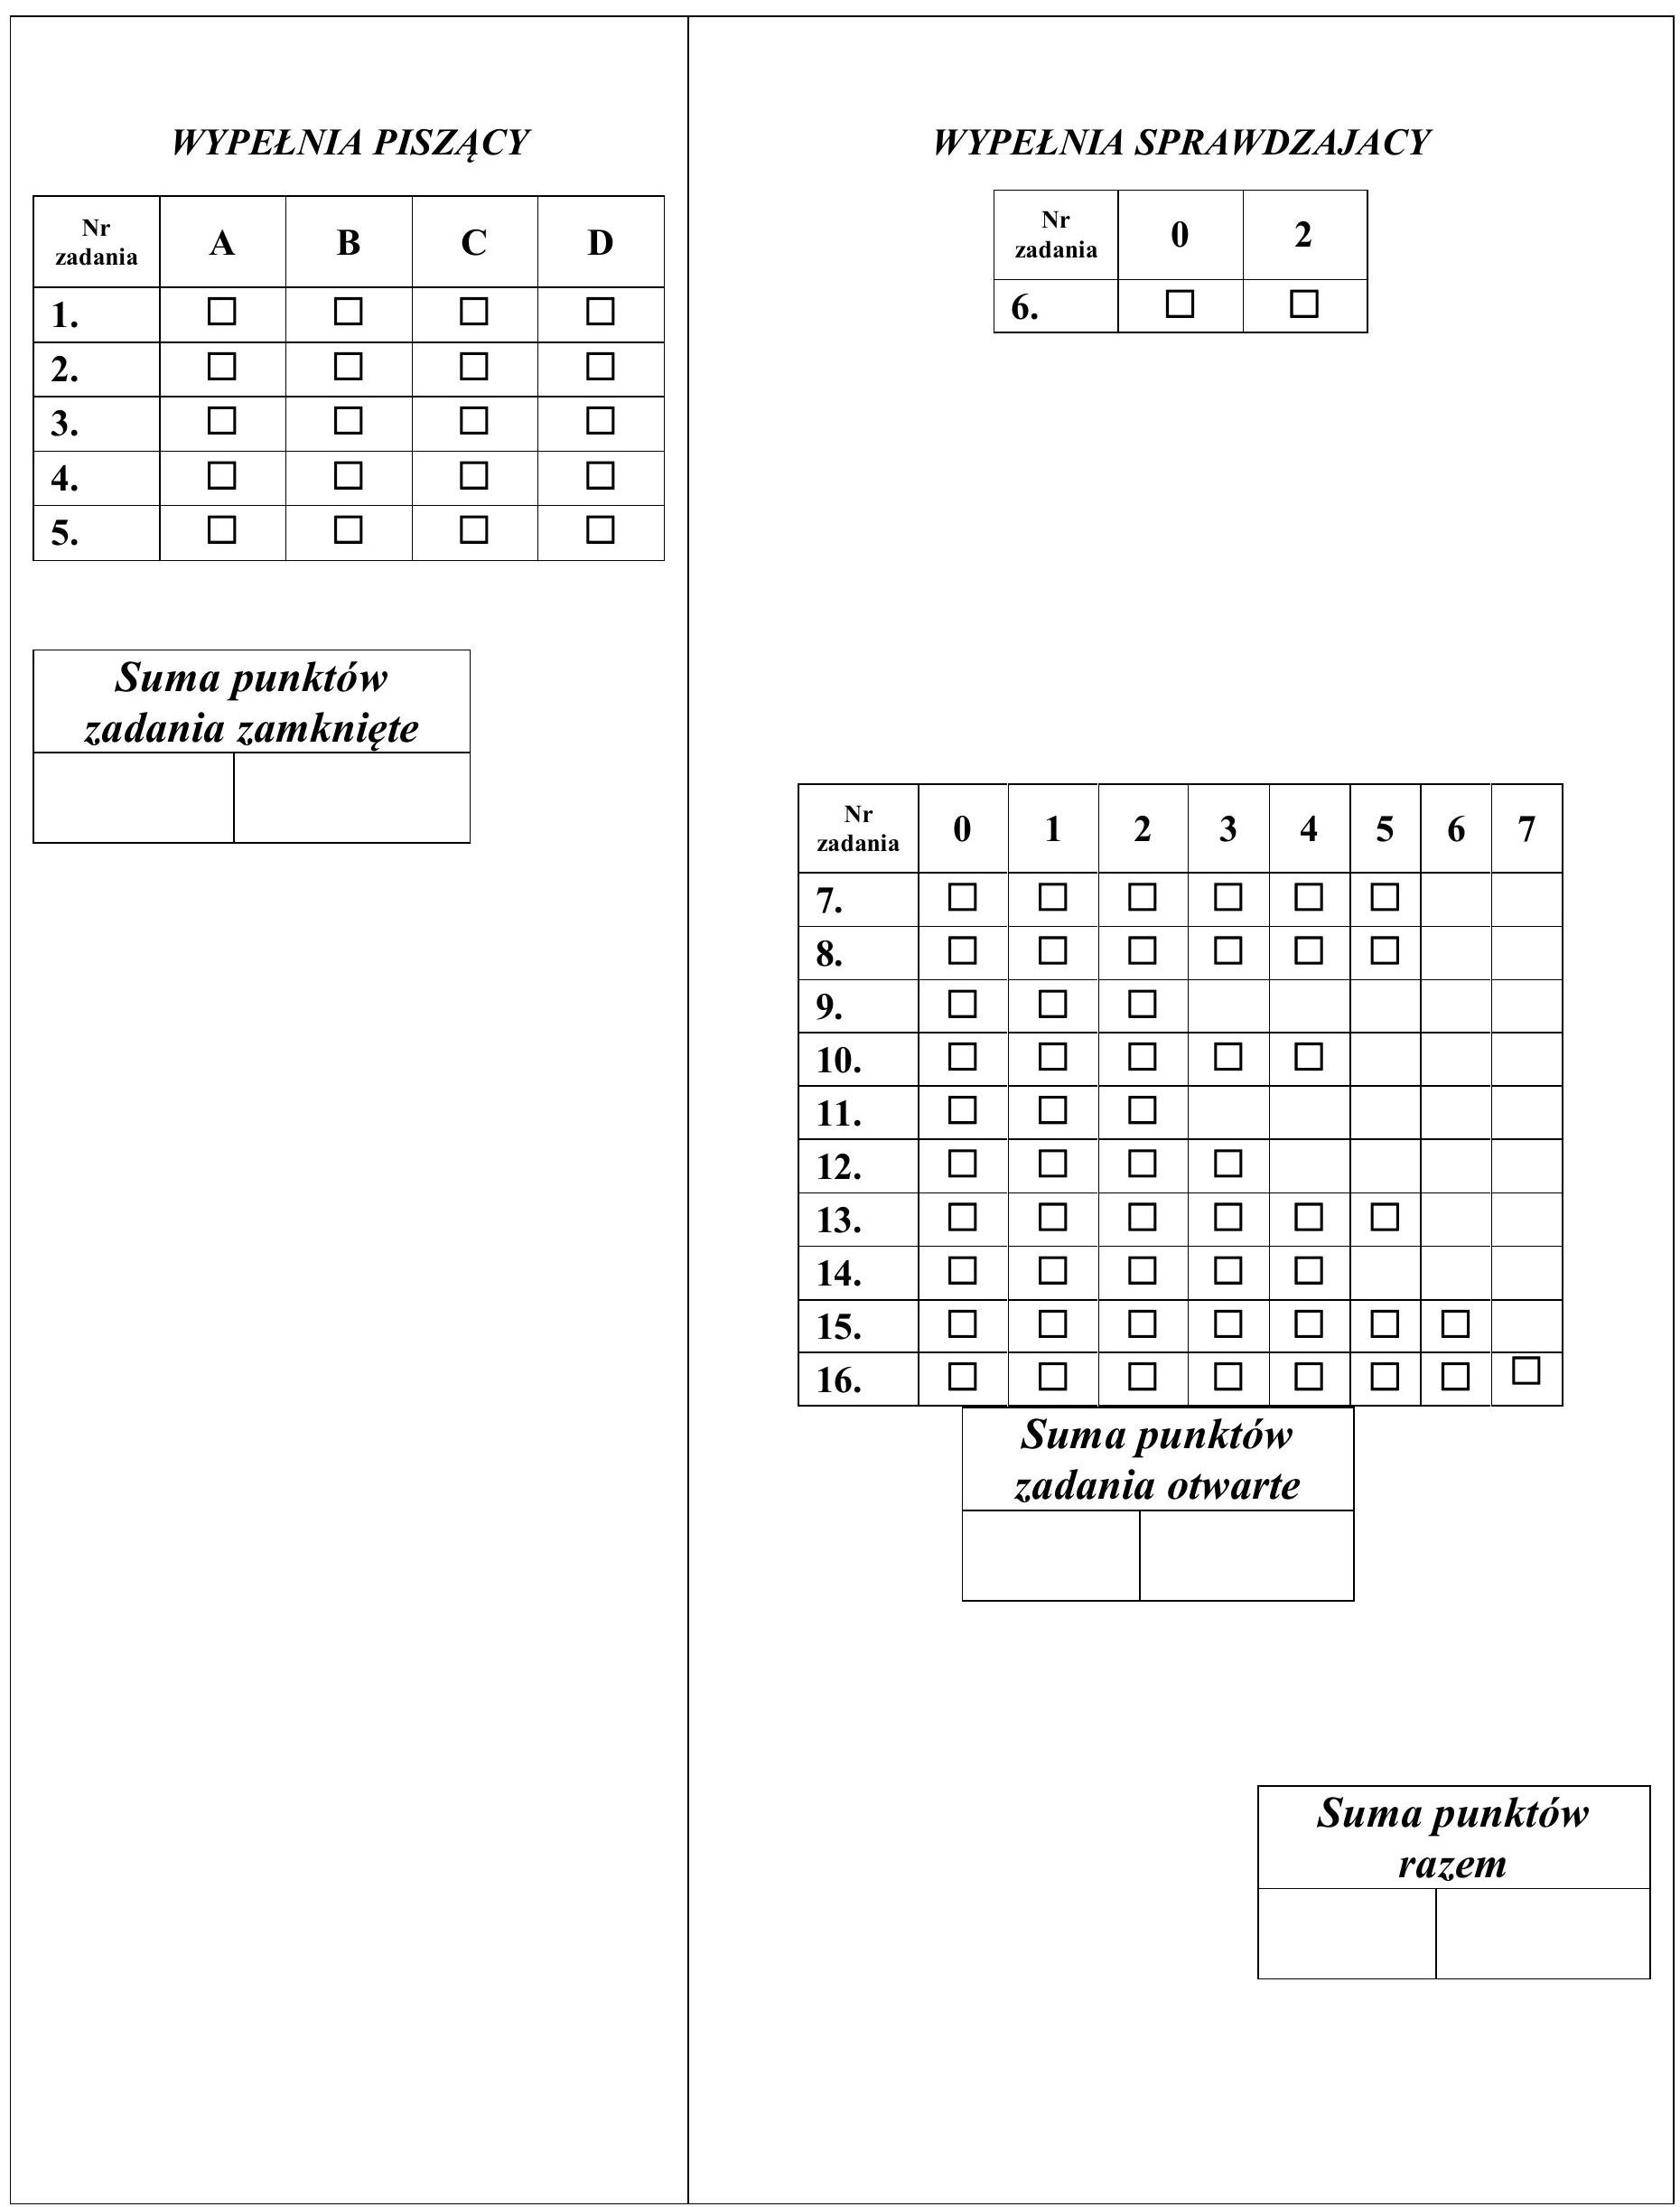
\includegraphics[max width=\textwidth]{2024_11_21_498389c978c770348ebcg-16}
\end{center}


\end{document}